\documentclass[a4paper, 10pt]{article}
\usepackage[utf8]{inputenc}
\usepackage[spanish]{babel}
\usepackage{graphicx}
\usepackage{geometry}
\usepackage{listings}
\usepackage{amsmath}
\usepackage{amsfonts}
\usepackage{amssymb}
\usepackage{caratula}

\newcommand{\Z}{\mathbb{Z}}
\def\code#1{\texttt{#1}}
\newcommand\tab[1][0.5cm]{\hspace*{#1}}

\geometry{a4paper, margin=0.7in}

\begin{document}
    %Caratula
    \pagenumbering{gobble}
    \newpage

    \begin{center}
        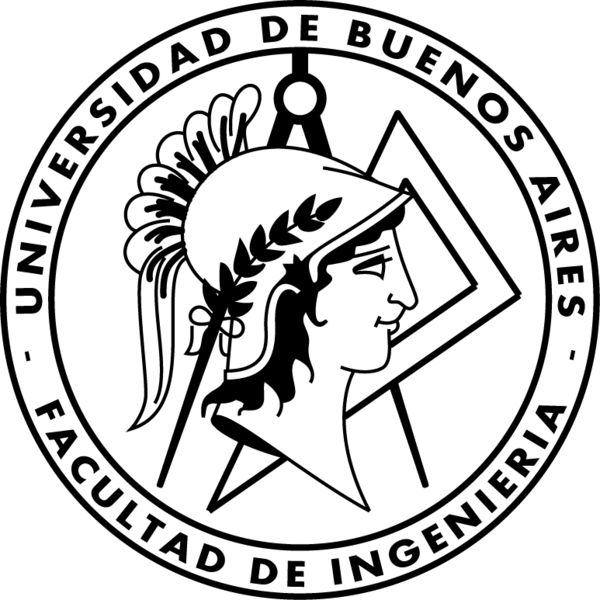
\includegraphics[width=5cm, height=5cm]{images/logo}
    \end{center}

    \materia{Teoría de Algoritmos I}
    \submateria{Primer Cuatrimestre 2017}
    \titulo{Trabajo Práctico 3}

    \integrante{Rodrigo De Rosa}{97799}{rodrigoderosa@outlook.com}
    \integrante{Marcos Schapira}{97934}{schapiramarcos@gmail.com}
    \integrante{Facundo Guerrero}{97981}{facundoiguerrero@gmail.com}
    \maketitle
    %Fin caratula
    %Table of contents
    \newpage
    \pagenumbering{roman}
    \tableofcontents
    %Fin table of contents
    %Informe
    \newpage
    \pagenumbering{arabic}

    \section{Programación Dinámica}
        En esta sección se analiza una solución al problema de la predcción de acciones a través
        de la programación dinámica.
        \subsection{Algoritmo}
        \tab El algoritmo utilizado para resolver el problema planteado esta basado en el algoritmo de kadane.
             Este busca la maxima suma de elementos contiguos dentro de un arreglo.
             \subsubsection{Funcionamiento}
              \tab Este algoritmo funciona de la siguiente forma:
              \begin{itemize}
                \item Inicializa un \code{día de compra}, un \code{día de venta}, un \code{día de compra auxiliar}, todos
                  como el primer dia. Tambien se inicializa una \code{ganancia máxima} y una \code{ganancia temporal},
                  ambas como 0 ya que, hasta el momento, el dia de compra es igual al dia de venta.

                \item Luego itera sobre todos los días (valores diferentes de acciones) verificando si
                  en el día actual( dia i ) es más o menos favorable comprar acciones que en el día en el
                  que se pretendía hacerlo hasta el momento( dia k ), determinando el \code{día de compra auxiliar}.
                  Esto asegura la obtencion de la mayor ganancia hasta el dia i-1.

                \item A partir del día que determinó, calcula la \code{ganancia temporal} como la ganancia que se obtendría
                  si las acciones fueran compradas en el \code{día de compra} y vendidas el \code{día actual}.
                  Luego se verifica si la \code{ganancia temporal} es mayor a la \code{ganancia máxima}.

                \item En tal caso, determina el \code{día de venta} como el actual, el \code{día de compra}
                  como el que previamente era el \code{día de compra auxiliar} y la \code{ganancia máxima} como
                  la que era la \code{ganancia temporal}.

                \item Al finalizar la iteración, queda determinado el \code{día de compra} más conveniente, el
                  \code{día de venta} más conveniente y la \code{ganancia máxima} obtenible.

                \item Dado que el algoritmo propuesto recorre una sola vez el arreglo, funciona en $O(n)$.
              \end{itemize}

            \subsubsection{Ecuación de recurrencia}
                Para la ecuación de recurrencia se plantea lo siguiente: \\
                \begin{itemize}
                  \item Para empezar, se debe tener en cuenta las siguientes consideraciones:

                  \item Para la resolución del algoritmo se utilizan las siguientes variables:
                  $ G_{M} $  = Ganancia Máxima, $G_{T}$ = Ganancia Temporal, $ D_{i}$ = Día actual,
                  $D_{V}$ = Día de Venta, $D_{C}$ = Día de Compra y $D_{CAux}$ = Día de Compra Auxiliar.

                  \item Para el paso i de la iteración, el $D_{CAux}$ se actualiza si $D_{i} < D_{C}$.
                  Esto se puedé hacer porque en el paso i ya se tiene la ganancia máxima calculada y guardada
                  en $G_{M}$. Como ahora se tiené un dia de compra mejor al que se teniá hasta el paso $i-1$,
                  la mejor ganancia que se pudó obtener hasta el paso $i-1$, es la que ya se obtuvó hasta el momento.
                  Entonces se lleván las nuevas ganancias en $G_{T}$ para poder observar si con el nuevo día de
                  compra se puede obtener una mejor ganancia.

                  \item La ganancia temporal se calcula como: $G_{T} = D_{i} - D_{CAux}$ y la ganancia máxima se calcula
                  como: $G_{M} = D_{V} - D{C}$. Entonces, se actualiza la ganancia máxima cuando $G_{M} < G_{T}$. Notar que en
                  dico caso tambien se actualizan los dias de compra y venta.

                  \item Entonces, se define $V_{i}$ como el valor de la accion en el día i.

                  \item Con las consideraciones anteriormente mencionadas, se puede notar que la ganancia en el dia $i$ es:
                  la ganancia del paso anterior, en el caso donde el valor de la acción es mayor en el día anterior que en el
                  día actual, o el máximo entre la ganancia del dia anterior y la ganancia del día actual.

                  \item Consideremos el siguiente caso de valores de acciones: [2,3,4,1,4,5]. Cuando $i=0$ el día de compra y el
                  día de venta son iguales entonces la ganancia es 0. Cuando $i=1$, ahora el día de venta es 1 y el día de compra
                  es 0, por lo tanto la ganancia es 1. Inductivamente sabemos que para $i=2$, la ganancia es 2. Pero en el caso en
                  que $i=3$ el día de compra pasa a ser 3, ya que la acción es mas barata, y la ganancia pasa a ser 0. Por eso, se
                  dicé que la ganancia del paso i es el maximo entre la ganancia del día anterior y la del día actual. En este caso
                  se puede observar que la ganancia del día anterior es 2 y la del día actual es 0, entonces corresponde la ganancia
                  del día anterior.

                  \item Entonces, se define la ganancia temporal para el paso i como: \\

                  \begin{center}
                    \tab\tab\tab$G_{M i,k}$ =
                    \begin{cases}
                        $G_{T} [i-1]$ & \mbox{si } $V_{i} \leqslant V_{i-1} $ \\
                        $V_{i} - D_{CAux}$ & \mbox{si } $V_{i} > V_{i-1}$
                    \end{cases}
                  \end{center}

                  \item Finalmente, vale notar que la ganancia máxima al finalizar la iteración será la ganancia temporal
                  calculada en el paso $n-esimo$.

                  \item Se ve claramente que el orden de dicho algoritmo es $O(n)$ ya que solamente se recorre el arreglo
                  una vez para obtener la máxima ganancia.
                \end{itemize}
    \newpage

    \section{Algoritmos Randomizados}
            En esta sección se analiza una solución al problema de hallar el corte global
        mínimo en un grafo no dirigido a través de un algoritmo randomizado.
        \subsection{Algoritmo}
                Para resolver este problema se utilizó el algoritmo de Karger descripto en
            la bibliografía proporcionada por la cátedra.
            \subsubsection{Funcionamiento}
                Sea el grafo $G = (E, V)$, el procedimiento del algoritmo es el siguiente:
                \begin{itemize}
                    \item Mientras $|V| > 2$:
                    \begin{itemize}
                        \item Se elige $e(u, v) \in E$ aleatoriamente.
                        \item Se crea un $w \in V$, el cual reemplaza tanto a $u$ como a $v$ en todas
                        las aristas en las que se encuentran. Es decir, $w$ puede tener más de una arista
                        que vaya a un mismo vértice $q \in V$.
                        \item Se elimina $e(u, v)$ de $E$.
                        \item Si existe alguna $e(v, v) \in E$ (arista de un vértice consigo mismo), se elimina.
                    \end{itemize}
                    \item Se devuelven las aristas que unen a esos dos vértices como el corte mínimo.
                \end{itemize}
            \subsubsection{Categoría de randomización}
                    Es un algoritmo \emph{Monte-Carlo} porque para algún orden de selección aleatoria
                de aristas, el corte obtenido \emph{no} es el mínimo. Es decir, es rápido siempre pero no siempre
                da resultados correctos. \\
                \tab La probabilidad de que este algoritmo devuelva un corte que sea mínimo es $p \geqslant \binom{n}{2}^{-1}$
                con $n = |V|$. Un dato adicional es que si el algoritmo se corre $T = \binom{n}{2}\ln{n}$ veces,
                la probabilidad de no encontrar un corte mínimo es $[1-p]^T \leqslant \dfrac{1}{n}$ en un tiempo
                $O(Tm) = O(n^2m\log{n})$ con $m = |E|$.
    \newpage

    \section{Algoritmos Aproximados}
        \tab En esta sección se analiza una solución al problema de la suma de subconjuntos
        a través de un algoritmo aproximado. Para resolver este problema se utilizó la
        estrategia polinómica descripta en la bibliografía proporcionada por la cátedra.
            \subsubsection{Funcionamiento}
                \tab El problema de la suma de subconjuntos (subset sum) consiste en, a partir de un conjunto S de enteros
                positivos y un target t también entero positivo, saber si existe algún subconjunto de S cuya suma sea
                exactamente t. Este problema es NP-Completo.\\
                \tab A partir de él se puede derivar a una aproximación completamente polinómica mediante el “recorte” o
                “trimming” de cada subconjunto que se va generando en el algoritmo exacto. Este mecanismo se sostiene de
                la idea de que si dos números pertenecen a S y tienen valores similares entonces no tiene mucho sentido
                mantener a ambos explícitamente (en referencia al algoritmo aproximado). Así es como mediante un parámetro
                de aproximación sigma tal que:
                                                            $0 < \sigma < 1$ \\
                \tab Se eliminan tantos elementos de S como sea posible ya que por cada elemento eliminado va a haber otro
                que pertenezca a S y lo represente. Así es como el algoritmo logra dado un conjunto S y un parámetro t
                devolver la mayor suma de elementos menor o igual a t. A la vez el algoritmo obtiene por parámetro a sigma,
                con lo cual la suma que devuelve está a un factor de $(1 + \sigma)$ del valor real.\\
            \subsubsection{Análisis del Algoritmo}
                \tab La tabla a continuación muestra resultados del algoritmo con $\sigma$ variables. A la vez los elementos
                en cada instancia y el valor de t fueron generados aleatoriamente. Z es el valor devuelto por el algoritmo.

                \begin{table}[h!]
                    \centering
                    \caption{Resultados para N = 350}


                    \begin{tabular}{c|c|c|c}
                        T & $\sigma$ & Zreal & Z real porcentual \\
                        \hline
                        2213 & 0,94 & 2211 & \%99,9 \\
                        \hline
                        2246 & 0,46 & 2245 & \%99,9 \\
                        \hline
                        2182 & 0,65 & 2182 & \%100 \\
                        \hline
                        2620 & 0,74 & 2618 & \%99,9 \\
                        \hline
                        173 & 0,62 & 172 & \%99,4 \\
                    \end{tabular}
                \end{table}

                \tab Como se puede apreciar, los porcentajes son extremadamente altos y caen dentro del factor esperado.
    \newpage

    \section{Ejecución de programas}
    \tab Para correr cada algoritmo, se debe ejecutar el archivo principal de cada uno.
    Esto se hace de la siguiente forma: \\
    \tab\tab En la carpeta \code{Programación Dinámica} abrir la consola y ejecutar \code{python main.py} \\
    \tab\tab En la carpeta \code{Algoritmos Randomizados} abrir la consola y ejecutra \code{python main.py} \\
    \tab\tab En la carpeta \code{Algoritmos Aproximados} abrir la consola y ejecutra \code{python main.py} \\

    %Fin informe
\end{document}
